% \appendix

\chapter{Appendix: Multiple Access and Scheduling Simulations}

\subsection{A3\_multiple\_access\_simulation.ipynb}

This Jupyter notebook demonstrates various multiple access techniques such as FDMA, TDMA, OFDMA, and NOMA using interactive Python visualizations. It includes practical implementations of:

\begin{itemize}
  \item Frequency division and time division allocation
  \item Subcarrier mapping in OFDMA
  \item Power-domain multiplexing in NOMA
  \item Basic scheduler logic for Round Robin and Proportional Fair algorithms
\end{itemize}

\noindent You can run and interact with the notebook directly via:

\begin{itemize}
  \item \textbf{Notebook GitHub link:} \url{https://github.com/your-repo/5G6G-course/blob/main/notebooks/A3_multiple_access_simulation.ipynb}
  \item \textbf{View online (via nbviewer):} \url{https://nbviewer.org/github/your-repo/5G6G-course/blob/main/notebooks/A3_multiple_access_simulation.ipynb}
\end{itemize}

\vspace{1em}
\subsection{SchedulerVisualizer.py (Streamlit App)}

To allow real-time interaction and exploration, we have also developed a dedicated Streamlit web app for this chapter.

This app provides:
\begin{itemize}
  \item Interactive sliders to simulate TDMA/FDMA/OFDMA with customizable users and resources
  \item A visual explanation of NOMA’s power domain allocation
  \item Simulated round-robin and proportional fair scheduler behavior
\end{itemize}

\noindent Run the app locally with:

\begin{verbatim}
streamlit run SchedulerVisualizer.py
\end{verbatim}

Or visit the hosted version here:

\begin{itemize}
  \item \textbf{Live app:} \url{https://your-app-hosting-url.com/SchedulerVisualizer}
\end{itemize}

\vspace{1em}
\subsection{Figures Used in This Chapter}

\vspace{1em}
\begin{figure}[H]
  \centering
  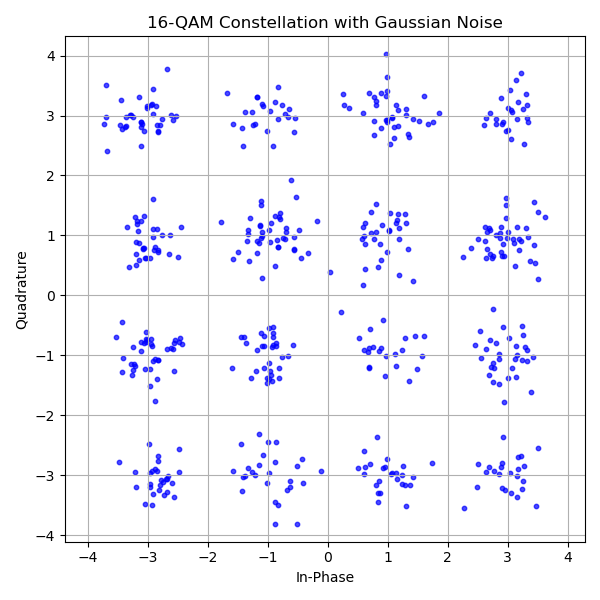
\includegraphics[width=0.85\textwidth]{./figures/modulation_constellation_example.png}
  \caption{Example modulation constellation diagram, used in Chapter 2 and referenced in scheduler visualizations.}
\end{figure}

\newpage
